\begin{figure}
  \centering
    \includegraphics[width=0.5\textwidth]{img/hand.eps}
  \caption{ReFlex Beta Hand}
  \label{fig:hand}
\end{figure}

\begin{figure}
  \centering
    \includegraphics[width=0.5\textwidth]{img/annotated_finger.eps}
  \caption{Close-up of a ReFlex Beta Hand finger}
  \label{fig:finger}
\end{figure}



\subsection{setup}

\subsubsection{Slave system}

In this setup the slave is characterized by a ReFlex Beta (RightHand Robotics) robotic hand. 

This device is made by the Harvard Biorobotics Lab and the Yale Grab Lab, it is a three fingered hand. Each finger is controlled by a single motor that pull the tendon in the finger, this tendon is connected to both the proximal and distal joint. This architecture allows each finger to shape itself to the object shape during the grasp. The fingers are distributed to optimize the object grasping, two finger are positioned on a side and the third is on the opposite one (Figure \ref{fig:hand}). 
During the experiments the hand must remain blocked in the initial position, the back looks downwards and the fingers upwards. 
This hand has a main particularity, on the surface are distributed 38 pressure sensors, for every finger there are 5 sensors on the proximal phalanx and 4 on the distal (Figure \ref{fig:finger}), the rest is on the palm. With this distribution it can do very precise pressure measures. 
The device is controlled by a Ethernet cable connected to a personal computer that handle every communication between the master and the slave system, the producers provide a ROS node to handle it.

\subsubsection{Master system}

The master has a little harder structure, it's mainly composed by a Leap Motion to recognize the user hand movements and a glove to give the feedback.

\textbf{\textit{Leap motion}} is an input device that allow to track the hand and fingers movements, is composed by two infrared (IR) cameras and three infrared leds, with this components it can calculate the distance of every point in his field of vision, from this map it can say if and where the user hands are. 
In \cite{weichert2013analysis} is presented a study of the precision and the stability of leap motion. For the purpose of this experiments the tracking provided by this device is enough accurate.

Instead the "glove" is homemade, it is composed by some \textbf{\textit{vibrating mini-motors}} fixed to the user hand with velcro straps and controlled by an Arduino Mega.

\textbf{\textit{Arduino}} is an open-source electronic prototyping platform that allow to create interactive electronic objects. It can be programmed through the Arduino IDE, that includes a GUI to write sketch (script in Arduino slang), the code compiler and a "programmer" to upload the compiled code on the device. Arduino is connected to the rest of the system through a serial cable.

Each mini-motor is connected to the Arduino through the PWM (Pulse Width Modulation), a signal switched between ON-OFF (5-0V), that returns a value between 0-255 according to the duty-cycle.
The mini-motors need of a simple electronic circuit to be controlled by a PWM signal (Figure \ref{fig:breadboard}).



\begin{figure}
  \centering
    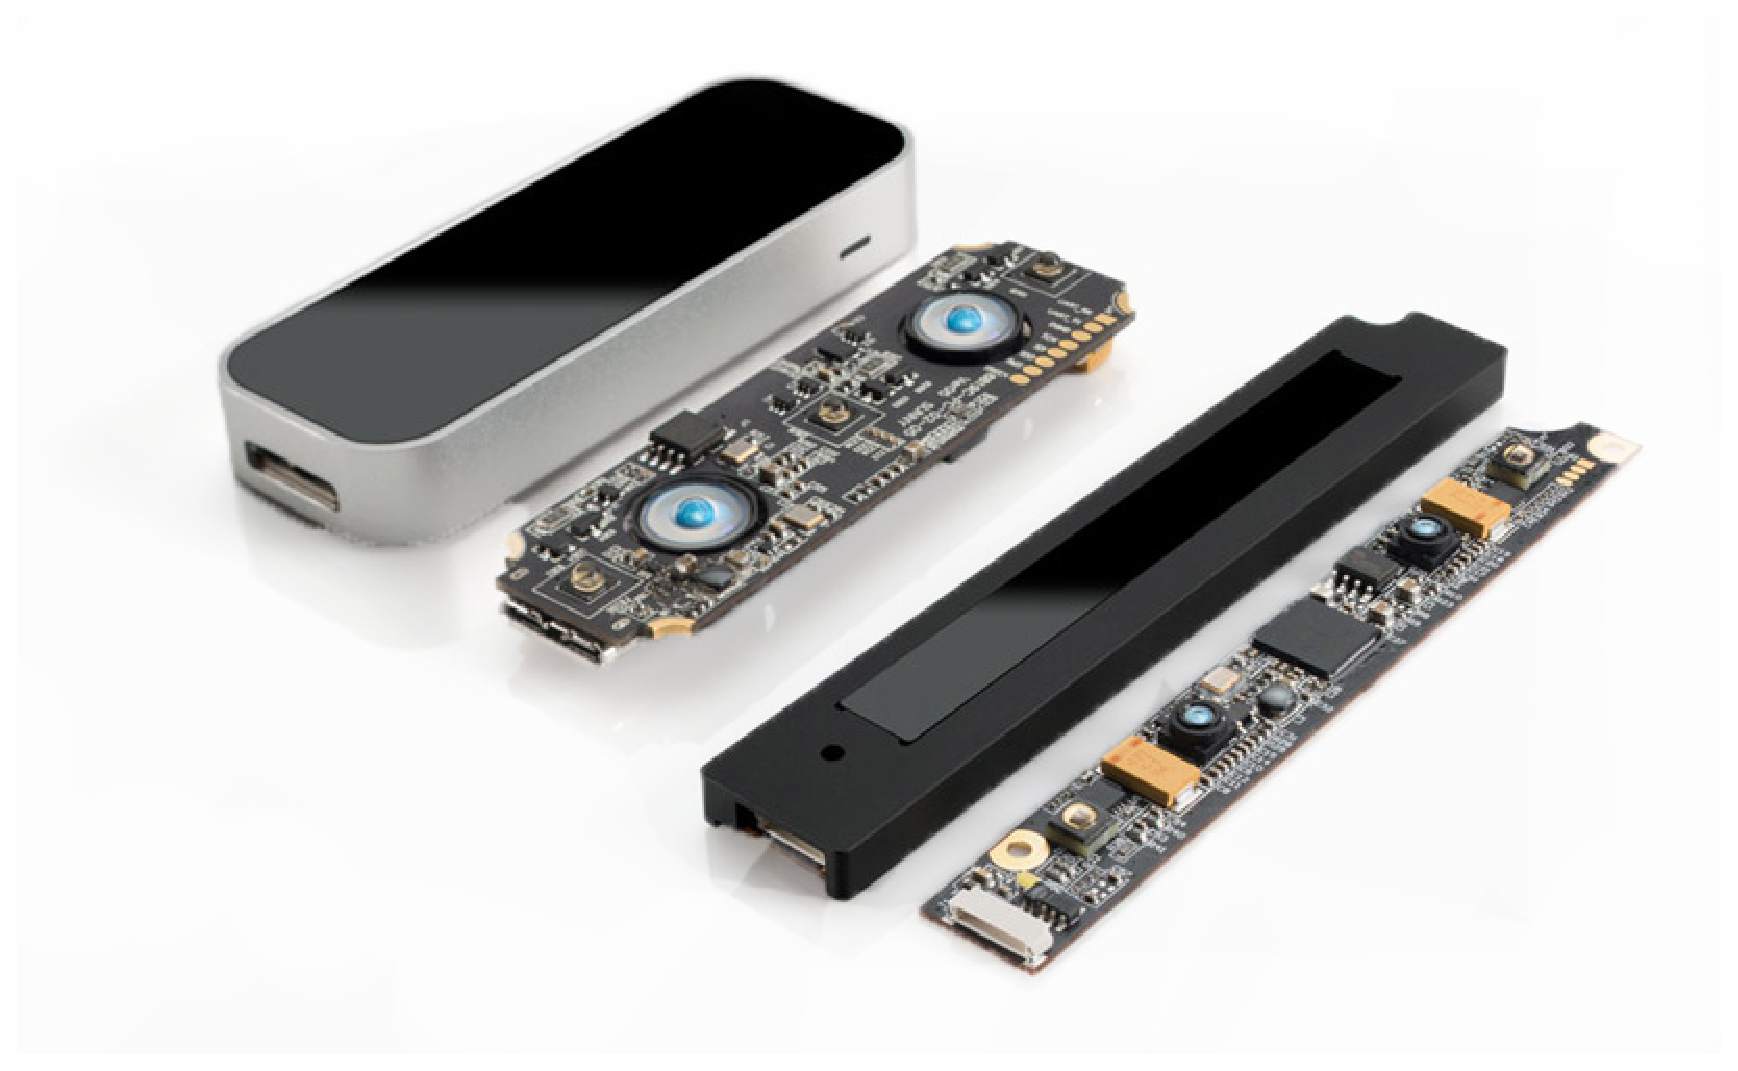
\includegraphics[width=0.5\textwidth]{img/leap_motion.eps}
  \caption{Leap motion}
  \label{fig:leap_motion}
\end{figure}

\begin{figure}
  \centering
    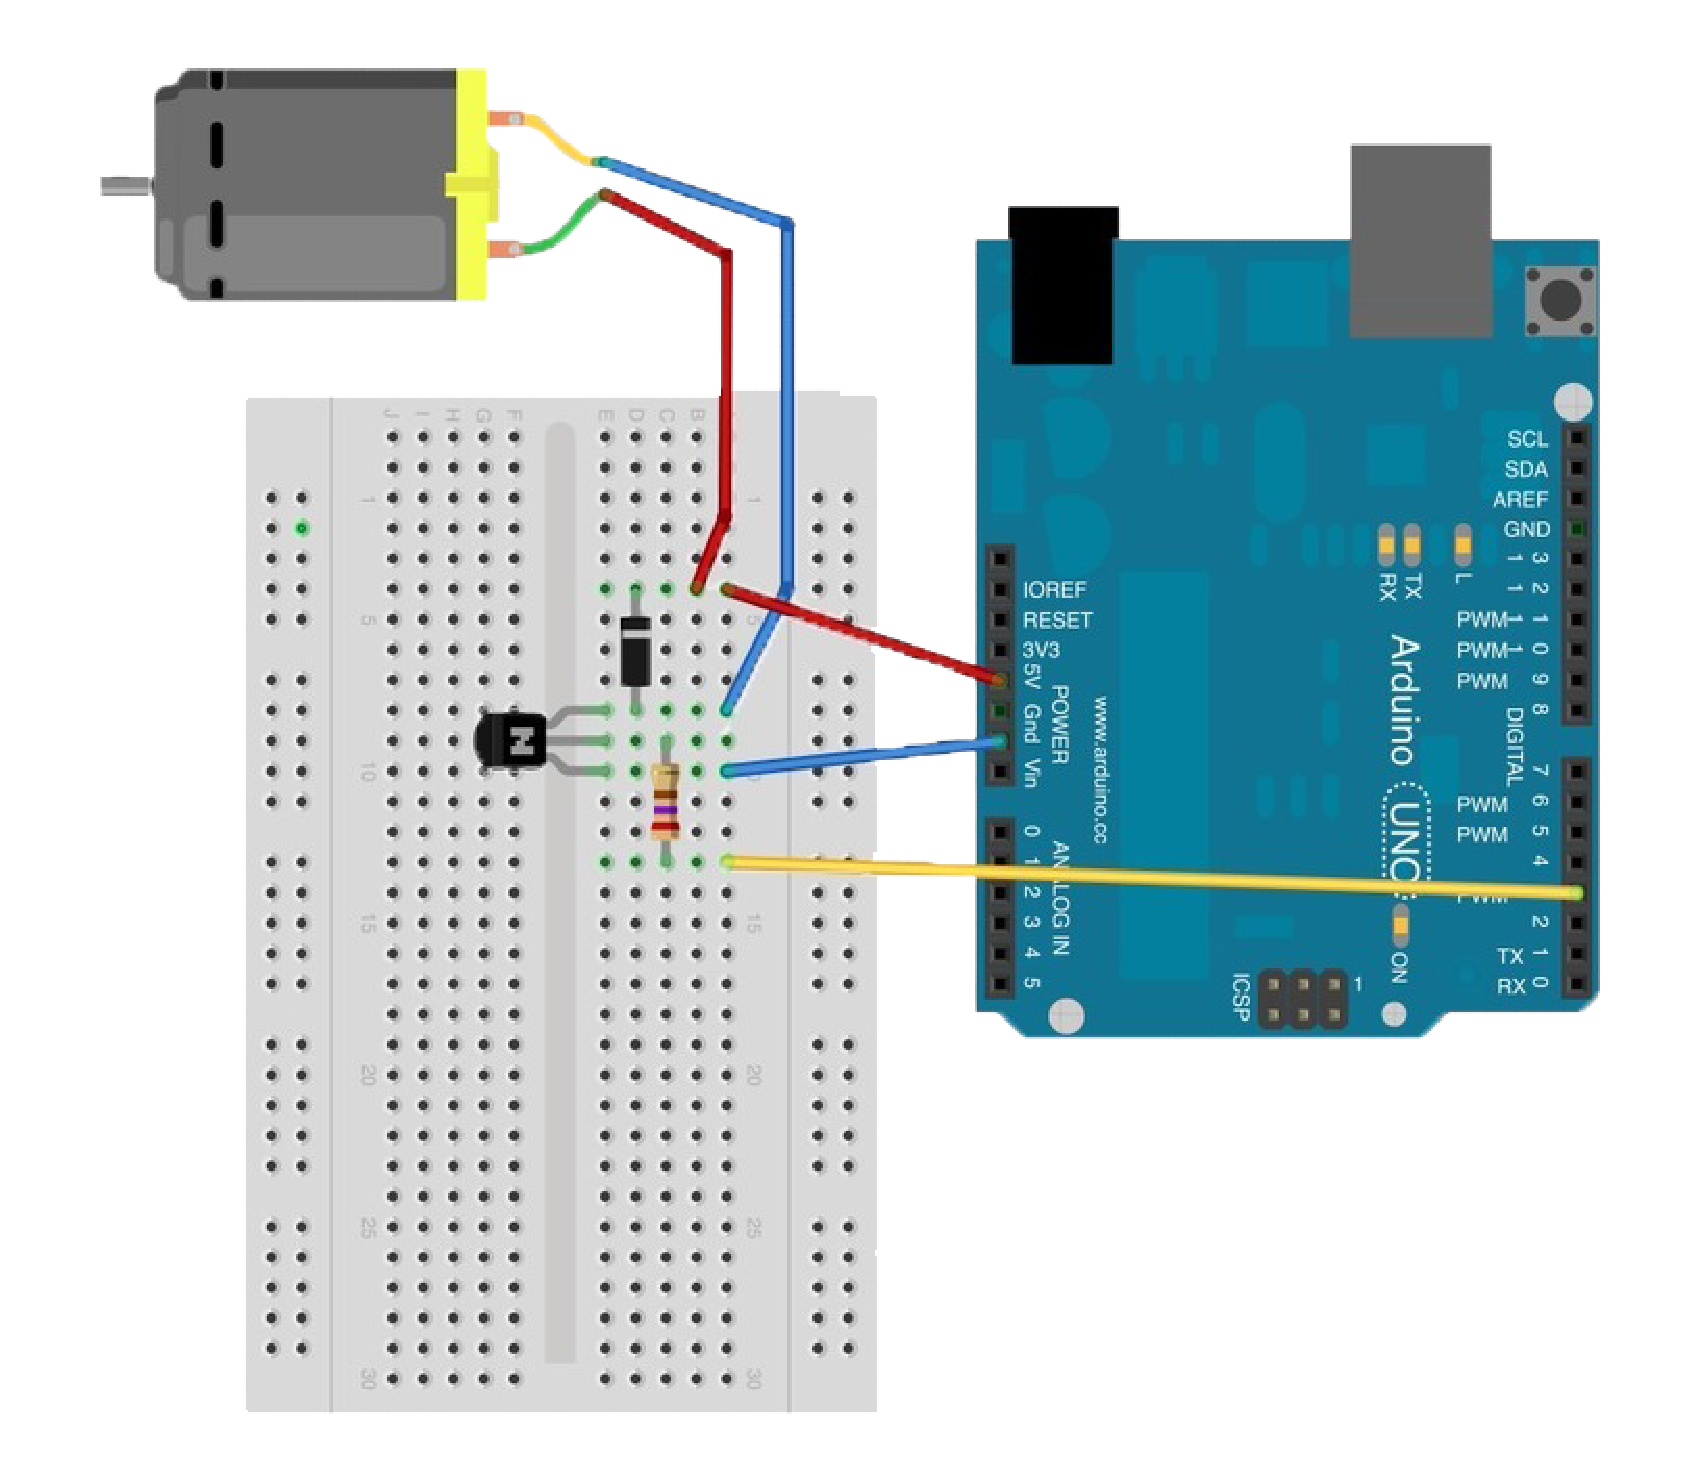
\includegraphics[width=0.5\textwidth]{img/breadboard.eps}
  \caption{Breadboard for vibratory mini-motor}
  \label{fig:breadboard}
\end{figure}

\subsection{Software architecture}